\documentclass{article}
\author{Alejandro Zubiri}
\date{Tue Oct 15 2024}
\title{Analisis}

\usepackage{amsmath}
\usepackage{amsthm}
\usepackage{physics}
\usepackage{amsfonts}
\usepackage{graphicx}

\graphicspath{ ../images/ }

\newtheorem*{lhopital}{Teorema}
\newtheorem*{taylor}{Teorema}

\begin{document}
\maketitle
\tableofcontents
\pagebreak
\section{Corolario del TVM}
Sea $g(x)=x$. Sea $f:[a,b] \to \mathbb{R}$, contínua en $[a,b]$ y derivable en $(a,b)$ 
$ \implies \exists c \in (a,b) /$
\begin{equation}
    \begin{split}
        (f(b)-f(a))g'(c) = (g(b) - g(a))f'(c)
    \end{split}
\end{equation}
que en este caso sería
\begin{equation}
    \begin{split}
        f(b)-f(a)=(b-a)f'(c)
    \end{split}
\end{equation}
Que reordenando es
\begin{equation}
    \begin{split}
        f'(c)= \frac{f(b)-f(a)}{b-a}
    \end{split}
\end{equation}
\section{Regla de L'Hôpital}
\begin{lhopital}[Regla de L'Hôpital]
    Sea $f,g$ derivables en un entorno de un punto $x=a$ y $\lim_{x \to a}f(x)=0$ y
    $\lim_{x \to a}g(x)=0$ y $\exists \lim_{x \to a} \frac{f'(x)}{g'(x)}$
\end{lhopital}
entonces
\begin{equation}
    \begin{split}
        \lim_{x \to a} \frac{f(x)}{g(x)}= \lim_{x \to a} \frac{f'(x)}{g'(x)}
    \end{split}
\end{equation}
\begin{proof}[Demostración]
    Supongamos que $f(a)=0$ y que $g(a)=0$
    \begin{equation}
        \begin{split}
            \frac{f(x)}{g(x)} = \frac{f(x)-f(a)}{g(x)-g(a)} = \frac{\frac{f(x)-f(a)}{x-a}}{\frac{g(x)-g(a)}{x-a}}
        \end{split}
    \end{equation}
    Si tomamos $\lim_{x \to a}$ en ambos lados
    \begin{equation}
        \begin{split}
            \lim_{x \to a} \frac{f(x)}{g(x)} = \lim_{x \to a} \frac{\frac{f(x)-f(a)}{x-a}}{\frac{g(x)-g(a)}{x-a}}
            = \lim_{x \to a} \frac{f'(x)}{g'(x)}
        \end{split}
    \end{equation}
    QED
\end{proof}
\section{Polinomio de Taylor}
\begin{proof}[Definición]
    Sea $f(x)$ una función derivable $n$ veces en el entorno de un punto $x_{0} \in (a,b)$.
    Se define Polinomio de Taylor de orden $n$ alrededor de un punto $x_{0}$:
    \begin{equation}
        \begin{split}
            Pn(f,x_{0})(x)= f(x_{0}) + \sum _{k=1}^n \frac{f^{k)} (x_{0})}{k!} (x-x_{0})^k
        \end{split}
    \end{equation}
\end{proof}
En caso de $x=x_{0}$ se denomina \textbf{serie McLaurin}.
\begin{taylor}[Teorema de Taylor]
    Sea $f(x)$ una función derivable $n+1$ veces. Sean $x,x_{0} \in  (a,b)$:
    \begin{equation}
        \begin{split}
            \exists \varepsilon \in (x,x_{0}) / f(x)-Pn(f,x_{0})(x)= \frac{f^{n+1}(\varepsilon)}{(n+1)!}(x-x_{0})^{n+1}
        \end{split}
    \end{equation}
\end{taylor}
\begin{proof}[Demostración]
    Supongamos que $x_{0}<x$ (el caso contrario es análogo). Vamos a definir una función
    auxiliar:
    \begin{equation}
        \begin{split}
            h(s)= f(s) + \sum ^n_{k=1} \frac{f^k (s)}{k!}(x-s)^{k}
        \end{split}
    \end{equation}
    Primero, $h(s)$ es contínua y derivable. Vamos a evaluar $h(s)$ en:
    \begin{itemize}
        \item $h(x)=f(x) + \sum ^n_{k=1} \frac{f^k (x)}{k!}(x-x)^{k}=f(x)$
        \item $h(x_{0})=f(x_{0})+\sum ^n_{k=1} \frac{f^k (x_{0})}{k!}(x-x_{0})^{k}= P_{n}(f,x_{0})(x)$
    \end{itemize}
    Ahora vamos a derivar la función:
    \begin{equation}
        \begin{split}
            h'(s) &= f'(s)+ \sum _{k=1} ^n \frac{f^{k+1}(s)}{k!} (x-s)^{k} +\sum ^n_{k=1}
            \frac{f^k (s)}{k!}k(x-s)^{k-1}\cdot -1\\
            &= f'(s)+ \sum _{k=1} ^n \frac{f^{k+1}(s)}{k!} (x-s)^{k} - 
            \sum ^n_{k=1} \frac{f^k (s)}{(k-1)!}(x-s)^{k-1}\\
            &= f'(s) + \sum _{k=1} ^n \frac{f^{k+1}(s)}{k!} (x-s)^{k} -
            f'(s ) -\sum ^n_{k=2} \frac{f^k (s)}{(k-1)!}(x-s)^{k-1}\\
            &= \sum _{k=1} ^n \frac{f^{k+1}(s)}{k!} (x-s)^{k}-\sum ^n_{k=2} \frac{f^k (s)}{(k-1)!}(x-s)^{k-1}\\
            &= \frac{f^{n+1}(s)}{n!}(x-s)^{n}
        \end{split}
    \end{equation}
    Vamos a crear una segunda función auxiliar:
    \begin{equation}
        \begin{split}
            g(s)= (x-s)^{n+1}
        \end{split}
    \end{equation}
    \begin{itemize}
        \item $g'(s)=-(n+1)(x-s)^{n}$
        \item $g(x) -g(x_{0})= (x-x)^{n+1} - (x-x_{0})^{n+1}= - (x-x_{0})^{n+1}$
        \item $g'(c)= -(n+1)(x-c)^{n}$
    \end{itemize}
    Si ahora aplicamos el teorema del valor medio, podemos afirmar que:
    \begin{equation}
        \begin{split}
            \exists c \in [x,x_{0}] / \quad \frac{h(x)-h(x_{0})}{g(x)-g(x_{0})} = \frac{h'(c)}{g'(c)}
        \end{split}
    \end{equation}
    Ahora evaluamos e igualamos:
    \begin{equation}
        \begin{split}
            \frac{h(x)-h(x_{0})}{g(x)-g(x_{0})} = \frac{f(x)- P_{n}(f,x_{0})(x)}{-(x-x_{0})^{n+1}}
        \end{split}
    \end{equation}
    \begin{equation}
        \begin{split}
            \frac{h'(c)}{g'(c)} &= \frac{\frac{f^{n+1}(c)}{n!}(x-c)^{n}}{-(n+1)(x-c)^{n}}\\
            &= \frac{f^{n+1}(c)}{-n!(n+1)} \\
            &= -\frac{f^{n+1}(c)}{(n+1)!}
        \end{split}
    \end{equation}
    \begin{equation}
        \begin{split}
            \frac{f(x)- P_{n}(f,x_{0})(x)}{-(x-x_{0})^{n+1}} &= -\frac{f^{n+1}(c)}{(n+1)!}\\
            f(x)- P_{n}(f,x_{0})(x) &= \frac{f^{n+1}(c)}{(n+1)!}(x-x_{0})^{n+1}
        \end{split}
    \end{equation}
    QED
\end{proof}
\section{Integrales - Técnicas de resolución}
\subsection{Cambio de variable}
Queremos integrales de la forma
\begin{equation}
    \begin{split}
        \int f(g(x))g'(x) \dd{x}
    \end{split}
\end{equation}
Podemos realizar la sustitución $t=g(x)$ y $\dd{t}=g'(x)\dd{x}$ para obtener
\begin{equation}
    \begin{split}
        \int f(g(x))g'(x) \dd{x} = \int f(t) \dd{t} = F(t)+C = F(g(x)) + C
    \end{split}
\end{equation}
\subsection{Integración por partes}
\begin{equation}
    \begin{split}
        \int u \dd{v} = u\cdot v - \int v \dd{u}
    \end{split}
\end{equation}
\begin{proof}[Demostración]
    Vamos a definir una función $h(x)$ tal que
    \begin{equation}
        \begin{split}
            h(x) = u(x)v(x)
        \end{split}
    \end{equation}
\end{proof}
Si tomamos su derivada, tenemos
\begin{equation}
    \begin{split}
        \dv{(u(x)v(x))}{x} = \dv{u}{x}v + u\dv{v}{x}
    \end{split}
\end{equation}
Si multiplicamos ambos lados por $\dd{x}$ tenemos que
\begin{equation}
    \begin{split}
        \dd{(u(x)v(x))} = v\dd{u} + u\dd{v}
    \end{split}
\end{equation}
Ahora podemos integrar para obtener
\begin{equation}
    \begin{split}
        \int \dd{(u(x)v(x))} &= \int v\dd{u} + u\dd{v}\\
        u(x)v(x) &= \int v\dd{u} + u\dd{v}
    \end{split}
\end{equation}
Si reordenamos, obtenemos que
\begin{equation}
    \begin{split}
        \int u \dd{v} = u\cdot v - \int v \dd{u}
    \end{split}
\end{equation}
QED
\subsection{Integración de funciones racionales}
Funciones de la forma
\begin{equation}
    \begin{split}
        \int f(x) \dd{x} = \int \frac{P(x)}{Q(x)} \dd{x}
    \end{split}
\end{equation}
Para las raíces que $Q(x) = 0$, tenemos dos casos:
\begin{itemize}
    \item Varias raíces: $(x-2)(x-3)$
    \item Valores repetidos: $(x-2)^{2}$
\end{itemize}
\subsubsection{Múltiples raíces}
\begin{equation}
    \begin{split}
        Q(x)= (x-a)(x-b)\dots (x-n)
    \end{split}
\end{equation}
Entonces tenemos
\begin{equation}
    \begin{split}
        \frac{P(x)}{(x-a)(x-b)\dots (x-n)} = \frac{A}{x-a} + \dots + \frac{N}{x-n}
    \end{split}
\end{equation}
\subsubsection{Raíces repetidas}
\begin{equation}
    \begin{split}
        Q(x) = (x-a)(x-b)\dots (x-b)^{n} \; / \; n>1
    \end{split}
\end{equation}
Entonces
\begin{equation}
    \begin{split}
        &\frac{P(x)}{(x-a)(x-b)\dots (x-b)^{n}} = \\
        &\frac{A}{x-a}+\dots + \frac{B}{(x-b)^n}
        + \frac{C}{(x-c)^{n-1}}+\dots + \frac{D}{x-d}
    \end{split}
\end{equation}
\subsection{Integrales trigonométricas}
\subsubsection{Funciones impares en el seno}
Se verifica que
\begin{equation}
    \begin{split}
        F(-\sin x) = -F(\sin x)
    \end{split}
\end{equation}
Realizaremos las sustituciones
\begin{equation}
    \begin{split}
        t &= \cos x\\
        \sin x &= \sqrt{1-t^{2}}\\
        \dd{x} &= \frac{- \dd{t}}{\sqrt{1-t^{2}}}
    \end{split}
\end{equation}
\subsubsection{Funciones impares en el coseno}
\begin{equation}
    \begin{split}
        F(\sin x, -\cos x) = -F(\sin x, \cos x)
    \end{split}
\end{equation}
Entonces sustituiremos
\begin{equation}
    \begin{split}
        t &= \sin x\\
        \cos x &= \sqrt{1-t^{2}}\\
        \dd{x} &= \frac{ \dd{t}}{\sqrt{1-t^{2}}}
    \end{split}
\end{equation}
\subsubsection{Funciones pares en ambos}
\begin{equation}
    \begin{split}
        F(-\sin x, \cos x) = F(\sin x, \cos x)
    \end{split}
\end{equation}
Cambiaremos
\begin{equation}
    \begin{split}
        t &= \tan x \\
        \sin x &= \frac{t}{t^{2}-1}\\
        \dd{x} &= \frac{ \dd{t}}{1+t^{2}}
    \end{split}
\end{equation}
\subsubsection{Caso general}
\begin{equation}
    \begin{split}
        \tan (\frac{x}{2}) &= t\\
        \sin x &= \frac{2t}{\sqrt{t^{2}+1}}\\
        \cos x &= \frac{1-t^{2}}{1+t^{2}}\\
        \dd{x} &= \frac{2}{1+t^{2}} \dd{t}
    \end{split}
\end{equation}
\section{Integral de Riemann}
\begin{center}
    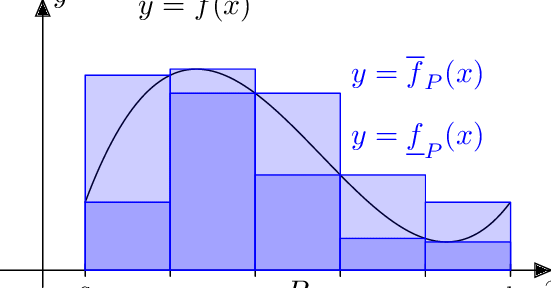
\includegraphics[scale=0.5]{../images/riemann.png}
\end{center}
Partimos de una función $f(x)>0 \forall x \in [a,b]$ y continua en todo el intervalo.\\
Dividimos el intervalo en particiones:
\begin{equation}
    \begin{split}
        [a,b]=[a,x_{1}] \cup [x_{1},x_{2}]\cup \dots\cup [x_{n-1}, b]
    \end{split}
\end{equation}
El área total es el área de cada pequeño intervalo.\\
Como $f(x)$ es continua, buscamos el máximo $M$ y el mínimo $m$ de cada intervalo. Definimos cada
$A_{i}$ como el área entre $x_{i-1}$ y $x_{i}$. Definimos como $R_{i}= M_{i} (x_{i}-x_{i-1})$ y
$r_{i} = m_{i}(x_{i}- x_{i-1})$. Se verifica siempre que:
\begin{equation}
    \begin{split}
        r_{i} \leq A \leq R_{i}
    \end{split}
\end{equation}
\begin{itemize}
    \item Aproximación por defecto:\\
    $s = \sum _{i=0}^n m_{i}(x_{i} - x_{i-1})$
    \item Aproximación por exceso:\\
    $S = \sum _{i=0} ^n M_{i}(x_{i}-x_{i-1})$
    \item Ahora se verifica también que $s \leq A \leq S$
\end{itemize}
\begin{proof}[Definición]
    Definimos como $p$ el conjunto de puntos que separan un intervalo. Una partición es más fina
    que otra si tiene menos puntos y si todos los puntos de la primera están contenidos en la segunda:
    \begin{equation}
        \begin{split}
            \forall x \in P_{1} \implies x \in P_{2}
        \end{split}
    \end{equation}
\end{proof}
Supongamos que la partición $P_{n}$ tiene $n$ puntos.\\
Cuando $n \to \infty$ la longitud del intervalo tiende a 0:
\begin{equation}
    \begin{split}
        n \to \infty \implies x_{i} -x_{i-1} \to 0
    \end{split}
\end{equation}
Por tanto
\begin{equation}
    \begin{split}
        \lim_{n \to \infty} s_{n} - S_{n} = \lim_{n \to \infty} \sum M_{i}(x_{i}-x_{i-1})-
        \sum m_{i}(x_{i}-x_{i-1})=0
    \end{split}
\end{equation}
y ahora
\begin{equation}
    \begin{split}
        \lim_{n \to \infty}S_{n} = \lim_{n \to \infty} s_{n}
    \end{split}
\end{equation}
Ahora, por la regla del sandwich:
\begin{equation}
    \begin{split}
        s_{n} \leq A \leq S_{n} \quad \implies \quad \lim_{n \to \infty}s_{n} = \lim_{n \to \infty}
        S_{n} = A
    \end{split}
\end{equation}
\begin{proof}[Definición]
    Sea $f(x)$ una función continua no negativa en $[a,b] \in \mathbb{R}$.\\
    La integral definida entre $a$ y $b$ de $f(x)$ es $ \int_{a}^b f(x) \dd{x}$ es el área
    comprendida entre $f(x)$, el eje de abscisas y las rectas $x=a$ y $x=b$. $a$ y $b$ son los
    límites de intergación.
\end{proof}
\subsection{Propiedades}
\begin{itemize}
    \item $ \int_{a}^a f(x) \dd{x}=0 \forall x \in Dom(f)$
    \item $f(x)>0 \forall x \in [a,b] \implies \int _{a}^b f(x)\dd{x}>0$
    \item $c \in [a,b] \implies \int_{a}^b f(x) \dd{x} = \int _{a}^c f(x) \dd{x} + \int _{c}^b f(x)\dd{x}$
    \item $ \int _{a}^b f(x) \dd{x} = - \int _{b}^a f(x) \dd{x}$ 
\end{itemize}
\begin{proof}[Teorema de Weierstrass]
    Si una función continua en un intervalo compacto (cerrado y acotado), sabemos que hay, al menos, dos puntos
    $x_{1},x_{2} \in [a,b]$ donde $f$ alcanza valores extremos absolutos:
    \begin{equation}
        \begin{split}
            f(x_{1}) \leq f(x) \leq f(x_{2})
        \end{split}
    \end{equation}
\end{proof}
\begin{proof}[Teorema del valor medio para integrales]
    Si una función es continua en $[a,b]$ entonces existe un punto:
    \begin{equation}
        \begin{split}
            c \in (a,b) / f(c)(b-a) = \int_{a}^b f(x) \dd{x}
        \end{split}
    \end{equation}
\end{proof}
\begin{proof}[Demostración]
    Sea $f(x)$ como en el enunciado:
    \begin{itemize}
        \item Si $f$ es constante en $[a,b]$:
        \begin{equation}
            \begin{split}
                \int _{a}^b f(x) \dd{x} = \int _{a}^b c \dd{x} = f(x)(b-a)
            \end{split}
        \end{equation}
    \end{itemize}
    \item Si no es constante, sean $M,m$ el valor máximo y mínimo, respectivamente. Sea $g(x) = m$:
    \item \begin{equation}
        \begin{split}
            m \leq f(x) \leq M \implies g(x) \leq f(x)
        \end{split}
    \end{equation}
    Por tanto
    \begin{equation}
        \begin{split}
            \int _{a}^b g(x) \dd{x} \leq \int _{a}^b f(x) \dd{x} \implies m(b-a) \leq \int _{a}^b f(x) \dd{x}
        \end{split}
    \end{equation}
    Y análogamente:
    \begin{equation}
        \begin{split}
            m(b-a) \leq \int _{a}^b f(x) \dd{x} \leq M(b-a)\\
            m \leq \frac{1}{b-a} \int _{a}^b f(x) \dd{x} \leq M
        \end{split}
    \end{equation}
    Ahora por Weierstrass, sabemos que $f$ alcanza el máximo y el mínimo en $[a,b]$,
    \begin{equation}
        \begin{split}
            \exists c \in (x_{1},x_{2}) \subset [a,b] / f(x_{1})=m \wedge f(x_{2})=M
        \end{split}
    \end{equation}
    Sea $f(c)=C$:
    \begin{equation}
        \begin{split}
            m \leq C \leq M
        \end{split}
    \end{equation}
    Si $C= \frac{1}{b-a} \int _{a}^b f(x) \dd{x} \implies  c \in [a,b]$, por tanto:
    \begin{equation}
        \begin{split}
            f(c)= \frac{1}{b-a} \int _{a}^b f(x) \dd{x}
        \end{split}
    \end{equation}
\end{proof}
\begin{proof}[Teorema fundamental del cálculo integral]
    Sea $f$ una función continua en $[a,b]$, y sea $F(x)= \int _{a}^x f(t) \dd{t} / x \in [a,b] \implies $ F es
    derivable y
    \begin{equation}
        \begin{split}
            F'(x)=f(x) \forall x \in [a,b]
        \end{split}
    \end{equation}
\end{proof}
\begin{proof}[Demostración]
    \begin{equation}
        \begin{split}
            F'(x) = \lim_{h \to 0} \frac{F(x+h) - F(x)}{h} = \lim_{h \to 0} \frac{ \int _{x}^{x+h} f(t) \dd{t}}{h}
        \end{split}
    \end{equation}
    Ahora podemos aplicar el teorema del valor medio para integrales:
    \begin{equation}
        \begin{split}
            \exists c \in [x,x+h] / f(c) \cdot h = \int _{x}^{x+h}f(t) \dd{t}
        \end{split}
    \end{equation}
    Por tanto
    \begin{equation}
        \begin{split}
            F'(x)= \frac{1}{h} \int _{x}^{x+h} f(t) \dd{t} = \lim_{h \to 0} \frac{f(c) \cdot h}{h}=\lim_{h \to 0}f(c)
            =f(x)
        \end{split}
    \end{equation}
\end{proof}
\begin{proof}[Corolario del TFC]
Sea $f$ una función continua en $[a,b]$:
\begin{equation}
    \begin{split}
        F(x)= \int _{g(x)}^{h(x)}f(t) \dd{t}
    \end{split}
\end{equation}
Si $g(x), h(x)$ son derivables entonces:
\begin{equation}
    \begin{split}
        F'(x)=f(h(x))h'(x) - f(g(x))g'(x)
    \end{split}
\end{equation}
\end{proof}
\begin{proof}[Teorema de Barrow]
    Sea una función continua $f$ y $F(x)$ una primitiva de $f(x)$:
    \begin{equation}
        \begin{split}
            \int _{a}^{b} f(x) \dd{x} = F(b)-F(a)
        \end{split}
    \end{equation}
\end{proof}
\begin{proof}[Demostración]
    Sea $g(x)= \int _{a}^{b} f(t) \dd{t}$. Por TFC, $g(x)$ es primitiva de $f(x)$:
    \begin{equation}
        \begin{split}
            g(x)-F(x) = c \in \mathbb{R} \implies g(x)= F(x)+c
        \end{split}
    \end{equation}
    En $x=a$:
    \begin{equation}
        \begin{split}
            g(x) = \int _{a}^{a}f(t) \dd{t}=0=g(a)= F(a)+c \implies c = -F(a)
        \end{split}
    \end{equation}
    En $x=b$:
    \begin{equation}
        \begin{split}
            g(b) = \int _{a}^{b}f(t) \dd{t}= F(b)+c = F(b)-F(a)
        \end{split}
    \end{equation}
    Por tanto
    \begin{equation}
        \begin{split}
            \int _{a}^{b} f(t) \dd{t} = F(b)-F(a)
        \end{split}
    \end{equation}
\end{proof}
\end{document}